\documentclass{beamer}
\usepackage[utf8]{inputenc}
\usepackage[T1]{fontenc}
\usepackage[ngerman]{babel}
\usepackage{graphicx}
\usepackage{gensymb}
\usepackage{bold-extra}
\usepackage{textcomp}
\usepackage{csquotes}
\usepackage{soul}
\usepackage{fancyvrb}

\input{../flat-blue-theme.inc}
\input{../footnotes.inc}

\setcounter{tocdepth}{1}

\setbeamercovered{invisible}
\beamertemplatenavigationsymbolsempty
\renewcommand*\insertshorttitle
{
	% To not count \pause as new frame. And also to make the package "appendixnumberbeamer" work.
	\makebox[0.94\textwidth]{\oldmacro\hfill\insertframenumber\,/\,\inserttotalframenumber}
}
\condensedToc

\title{OpenStreetMap}
\subtitle{What is that and how can I contribute?}
\author{Hauke Stieler\\4stieler@inf}
\titlegraphic{
\includegraphics[width=1.5cm,keepaspectratio]{images/openstreetmap-logo.jpg}}
\date{\today}

\begin{document}
	\maketitle
	
	\begin{frame}
		\tableofcontents
	\end{frame}
	
	\section{Geodata basics}
	
		\subsection{Geodata basics}
	
		\begin{frame}{What is \enquote{geodata}?}
			\begin{definition}
				Information with geographical reference.
			\end{definition}
			\pause
			Anything with a coordinate, geometry or other kind of geographical information:
			\begin{itemize}
				\item house with address\pause
				\item measured temperature at certain coordinate\pause
				\item aerial imagery\pause
				\item recorded bicycle track\pause
				\item ...
			\end{itemize}
		\end{frame}
		
		\begin{frame}{Formats}
			Main categories:
			\begin{itemize}
				\item vector files\pause
				\item raster files\pause
				\item database \textleftarrow\ OSM\pause
				\item web services
			\end{itemize}
		\end{frame}
		
		\begin{frame}{File and web formats}
			\begin{columns}[t]
				\begin{column}{0.47\textwidth}
					Vector formats
					\begin{itemize}
						\item GeoJSON
						\item GeoPackage, SpatiaLite
						\item Shapefile
						\item KML, GML, WKT, OSM
					\end{itemize}
					\pause
					Raster formats
					\begin{itemize}
						\item GeoTIFF
						\item netCDF, JPEG2000
					\end{itemize}
					\pause
				\end{column}
				\begin{column}{0.53\textwidth}
					Web services:
					\begin{itemize}
						\item OGC (WMS, WMTS, WFS, ...)
						\item XYZ-tiles
						\item ArcGIS
					\end{itemize}
				\end{column}
			\end{columns}
		\end{frame}
		
		\begin{frame}{Vector data (GeoJSON)}
			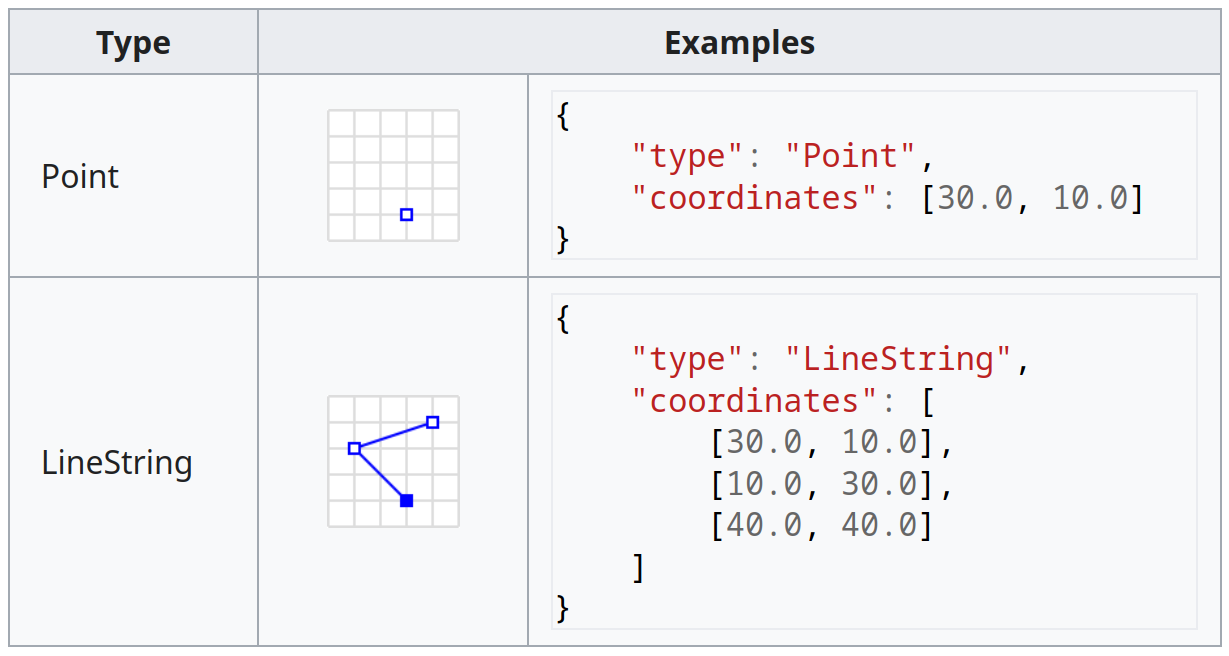
\includegraphics[width=\textwidth]{images/geodata-vector-1.png}\footnote{\href{https://en.wikipedia.org/wiki/GeoJSON}{Wikipedia -- GeoJSON}}
		\end{frame}
		
		\begin{frame}{Vector data (GeoJSON)}
			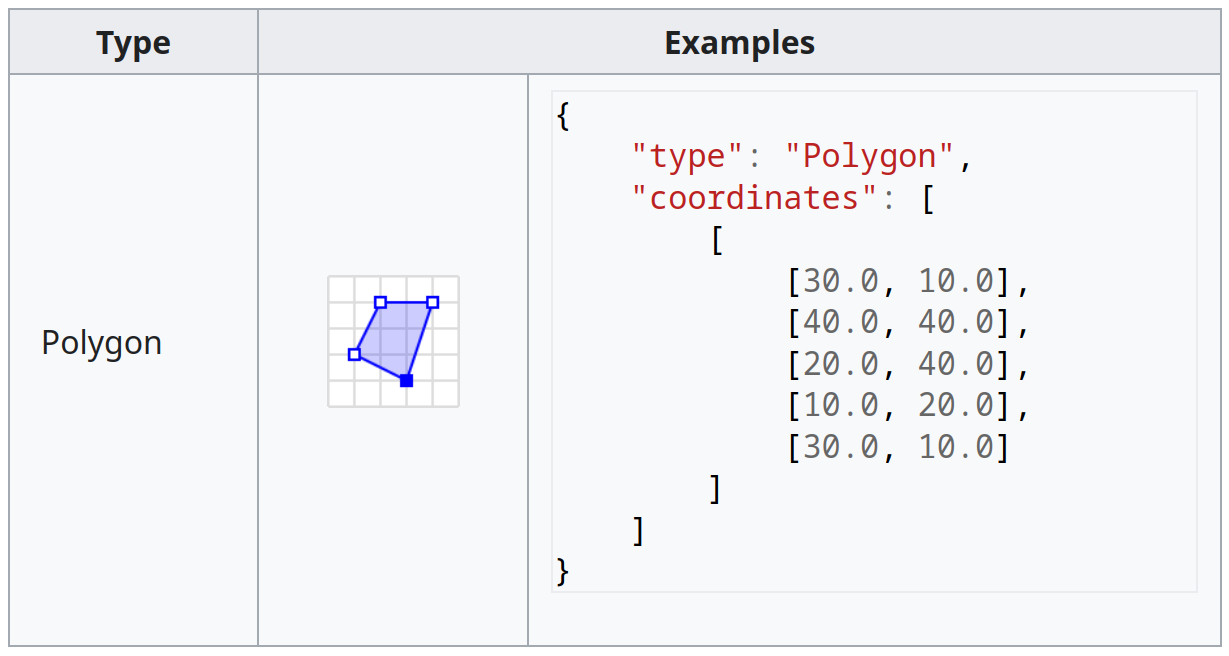
\includegraphics[width=\textwidth]{images/geodata-vector-2.png}\footnote{\href{https://en.wikipedia.org/wiki/GeoJSON}{Wikipedia -- GeoJSON}}
		\end{frame}
		
		\begin{frame}{Attributes / properties}
			\begin{itemize}
				\item add information to geometry
				\begin{itemize}
					\item geometry: \textit{Where} is it?
					\item attributes: \textit{What} is it?
				\end{itemize}\pause
				\item usually key-value-pairs\pause
				\item formats restrict types and values
			\end{itemize}
			\pause
			\vspace{0.5cm}
			\begin{center}
				geometry + attributes = feature
			\end{center}
		\end{frame}
		
	\section{OSM overview}
	
		\begin{frame}
			\tableofcontents[currentsection]
		\end{frame}
	
		\subsection{Imagine ...}
			
			\begin{frame}{... you want to use a map that is ...}
				\begin{itemize}
					\item up to date\pause
					\item contains all sort of stuff (infrastructure, vegetation, POIs, ...)\pause
					\item routable (car, bicycle, foot, train, ...)
				\end{itemize}
			\end{frame}
			
			\begin{frame}{... constantly changing areas}
				\begin{center}
					\textbf{Example:}\\
					Construction of A7\\
					{\tiny (Hamburg-Stellingen, Germany)}
				\end{center}
			\end{frame}
		
			\begin{frame}{... unusual use cases}
				\begin{itemize}
					\item routing for canoes
					\item search POIs by accessibility
					\item research analysis
				\end{itemize}
			\end{frame}
		
			\begin{frame}{... you want to create/print/host/use maps}
				\begin{itemize}
					\item on invitation card to weddings/birthday/party/...
					\item in presentations
					\item for private purposes (e.g. cycling)
					\item in commercial uses
					\begin{itemize}
						\item on websites
						\item maps in bus/train stops
						\item public city map
					\end{itemize}
				\end{itemize}
			\end{frame}
		
			\begin{frame}{... a solution for all of this}
				\begin{center}
					And yes, it exists:\\
					\hfill\\
					\textbf{OpenStreetMap}\\
					{\tiny (short: OSM)}
				\end{center}
			\end{frame}

		\subsection{What is OSM?}
	
			\begin{frame}
				\begin{itemize}
					\item free\footnote{\textit{free} as in \textit{free}dom} project collecting \textbf{free accessible} geodata
					\item open database for geodata
					\item ODC-ODbL
					\begin{itemize}
						\item OpenDataCommons Open Database License
						\item Replaced CC BY-SA 2.0 {\tiny (share alike \& attribution)}
					\end{itemize}\pause
					\item OpenStreetMap Foundation (OSMF)
					\item financed by donations, conferences and memberships\footnote{374k income in 2022}
					\item history
					\begin{itemize}
						\item started in 2004
						\item API basically unchanged since 2009
						\item 1 mio. contributors in 2013
						\item approx. 11mio. contributors in 2024\footnote{Doubled since last KBS WTF?!}
					\end{itemize}
				\end{itemize}
			\end{frame}

			\begin{frame}{Why OSM?}
				\begin{columns}[t]
					\begin{column}{0.5\textwidth}
						Proprietary maps
						\begin{itemize}
							\item often old and faulty\pause
							\item focus on cars and traffic\pause
							\item license problems all over the place\pause
							\item no access to raw data
							\item no contribution possible
						\end{itemize}
					\end{column}
					\pause
					\begin{column}{0.5\textwidth}
						Official data
						\begin{itemize}
							\item often old and faulty\pause
							\item not always usable data (e.g. for routing)\pause
							\item not always free/open\pause
							\item no contribution possible
						\end{itemize}
						\pause
						But:\\
						More and more open and often access to raw data
					\end{column}
				\end{columns}
			\end{frame}
			
			\begin{frame}{Excursion: Open Data in Germany}
				Moving towards:
				\begin{itemize}
					\item legally open/accessible
					\begin{itemize}
						\item open license: CC BY-SA 4.0, DL-DE BY 2.0, CC0
					\end{itemize}\pause
					\item technically open/accessible
					\begin{itemize}
						\item web API (OGC compliant)
						\item professional formats (no \texttt{.pdf} and \texttt{.xlsx} WTF?!)
					\end{itemize}
				\end{itemize}
				\pause
				\vspace{0.5cm}
				Access via web APIs/interfaces, e.g. \href{https://www.geoportal.de/}{geoportal.de}
			\end{frame}
			
			\begin{frame}{Statistics}
				\begin{itemize}
					\item 11 mio. contributors
					\item 40,000 monthly contributors
					\item 110 mio. changes per month\footnote{2750 edits per contributor per month}
					\item 8.8 Bn. points, 1 Bn. lines/polygons, 11 mio. relations
					\item tile server: 50,000 requests/min
				\end{itemize}
			\end{frame}
			
			\begin{frame}{Stuff by the OSMF}
				\begin{itemize}
					\item database, backup servers, mirrors
					\item API server
					\item tile rendering
					\begin{itemize}
						\item Live rendering! Tiles are updates nearly instantly!
						\item CDN
					\end{itemize}
					\item geocoder (search service)
					\item routing
					\item internal services
					\begin{itemize}
						\item data statics (taginfo)
						\item query server (overpass)
						\item wiki
						\item git, trac, irc, BBB, ......
					\end{itemize}
				\end{itemize}
				\pause
				\textrightarrow\ \href{https://hardware.openstreetmap.org/}{hardware.osm.org}
			\end{frame}
			
			\begin{frame}{Stuff by someone else}
				\begin{itemize}
					\item maps
					\begin{itemize}
						\item \href{https://map.openseamap.org/?zoom=13.5\&lon=9.96566\&lat=53.52952}{OpenSeaMap}
						\item \href{https://openbeermap.github.io/\#17/53.54957/9.96370}{OpenBeerMap}
						\item \href{https://opentopomap.org}{OpenTopoMap}
						\item .....
					\end{itemize}\pause
					\item create your own map: \href{https://print.get-map.org/}{MyOSMatic}\pause
					\item getting the data
					\begin{itemize}
						\item \href{https://overpass-turbo.eu/}{overpass} with filtering
						\item larger datasets: \href{http://download.geofabrik.de/}{Geofabrik GmbH} <3
					\end{itemize}
					\item tools, frameworks, libraries, etc.
				\end{itemize}
				\pause
				\vspace{0.5cm}
				Many, many, many more \textrightarrow\ \href{https://wiki.openstreetmap.org/wiki/List\_of\_OSM-based\_services}{OSM-wiki: List of OSM-based services}
			\end{frame}
			
		\subsection{Applications}
			
			\begin{frame}{OpenStreeMap website (last KBS)}
				\begin{center}
					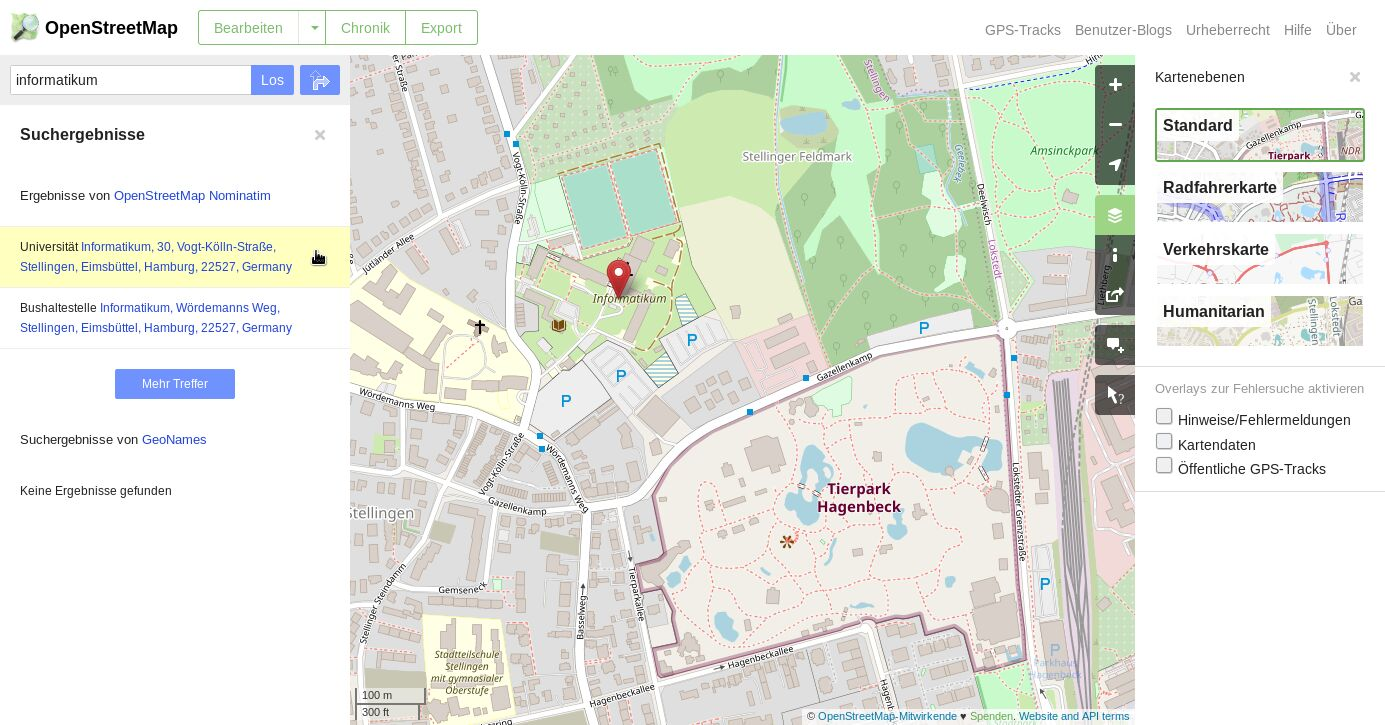
\includegraphics[height=0.7\textheight]{images/osm-website-old.jpg}\\
					\url{https://osm.org}
				\end{center}
			\end{frame}
			
			\begin{frame}{OpenStreeMap website}
				\begin{center}
					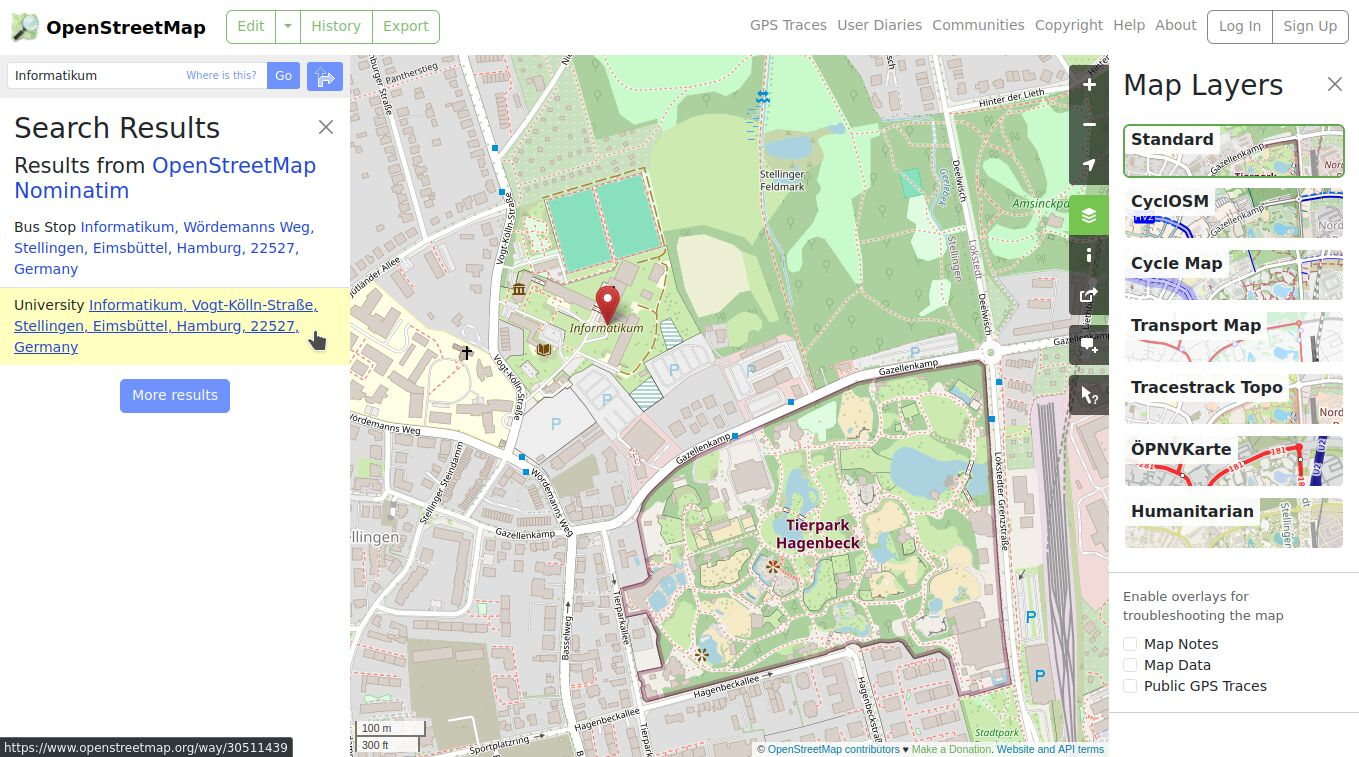
\includegraphics[height=0.7\textheight]{images/osm-website.jpg}\\
					\url{https://osm.org}
				\end{center}
			\end{frame}
			
			\begin{frame}{OpenRouteService}
				\begin{center}
					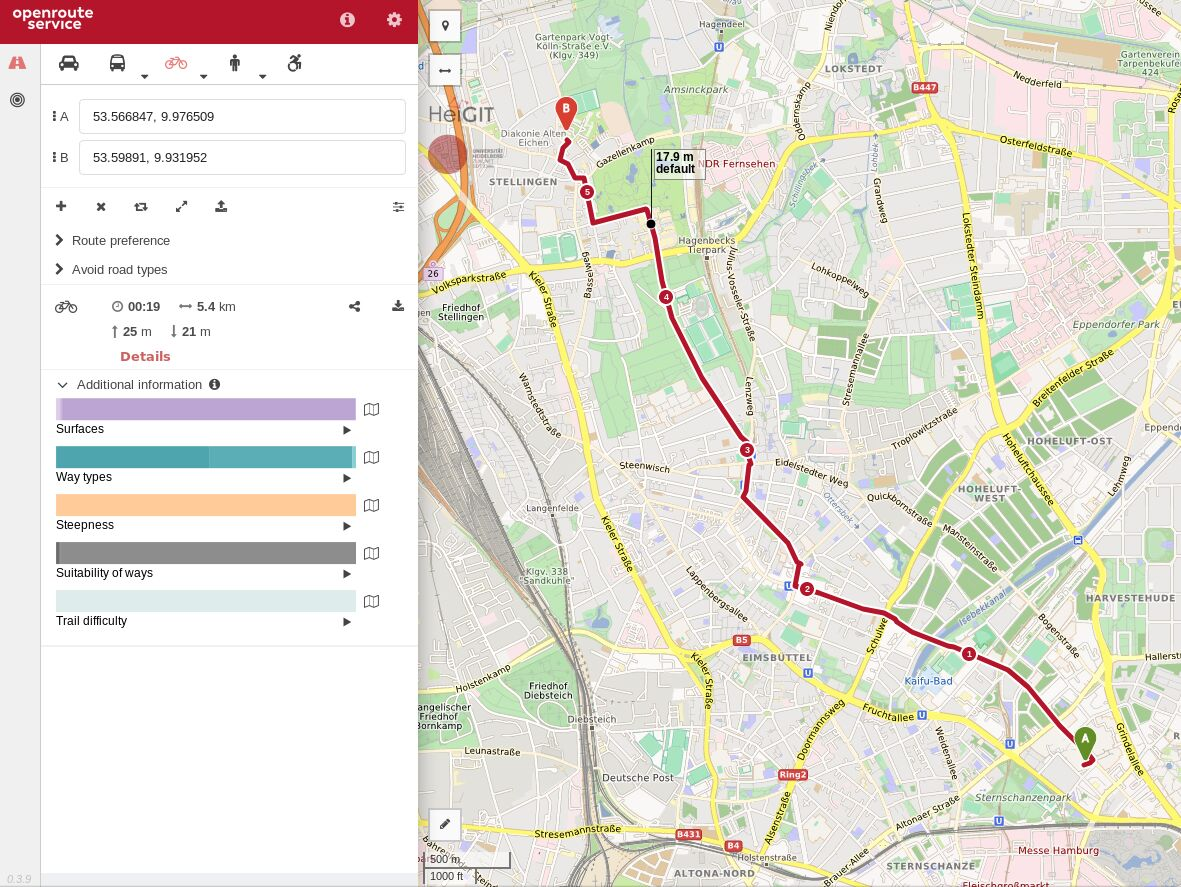
\includegraphics[height=0.7\textheight]{images/openrouteservice.jpg}\\
					\url{https://maps.openrouteservice.org}
				\end{center}
			\end{frame}
			
			\begin{frame}{OpenTopoMap website}
				\begin{center}
					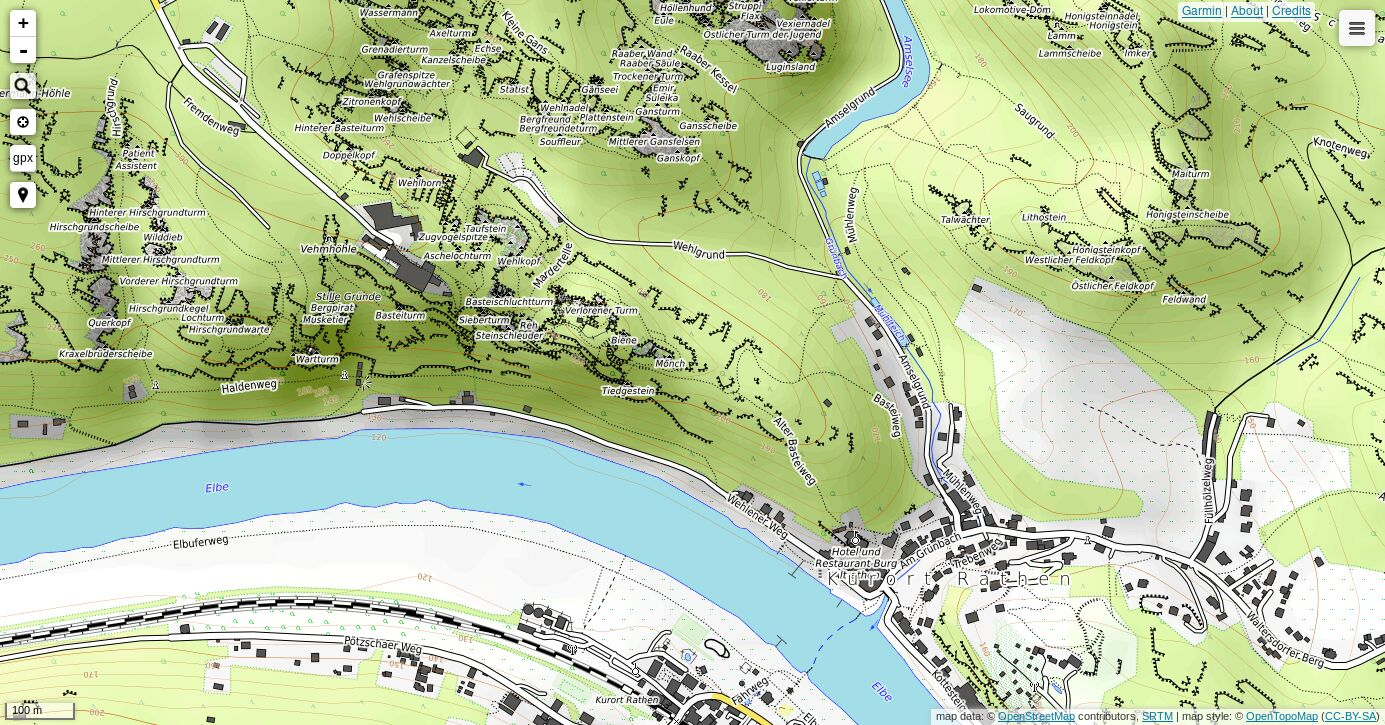
\includegraphics[height=0.7\textheight]{images/opentopomap-website.jpg}\\
					\url{https://opentopomap.org}
				\end{center}
			\end{frame}
			
			\begin{frame}{Wheelmap}
				\begin{center}
					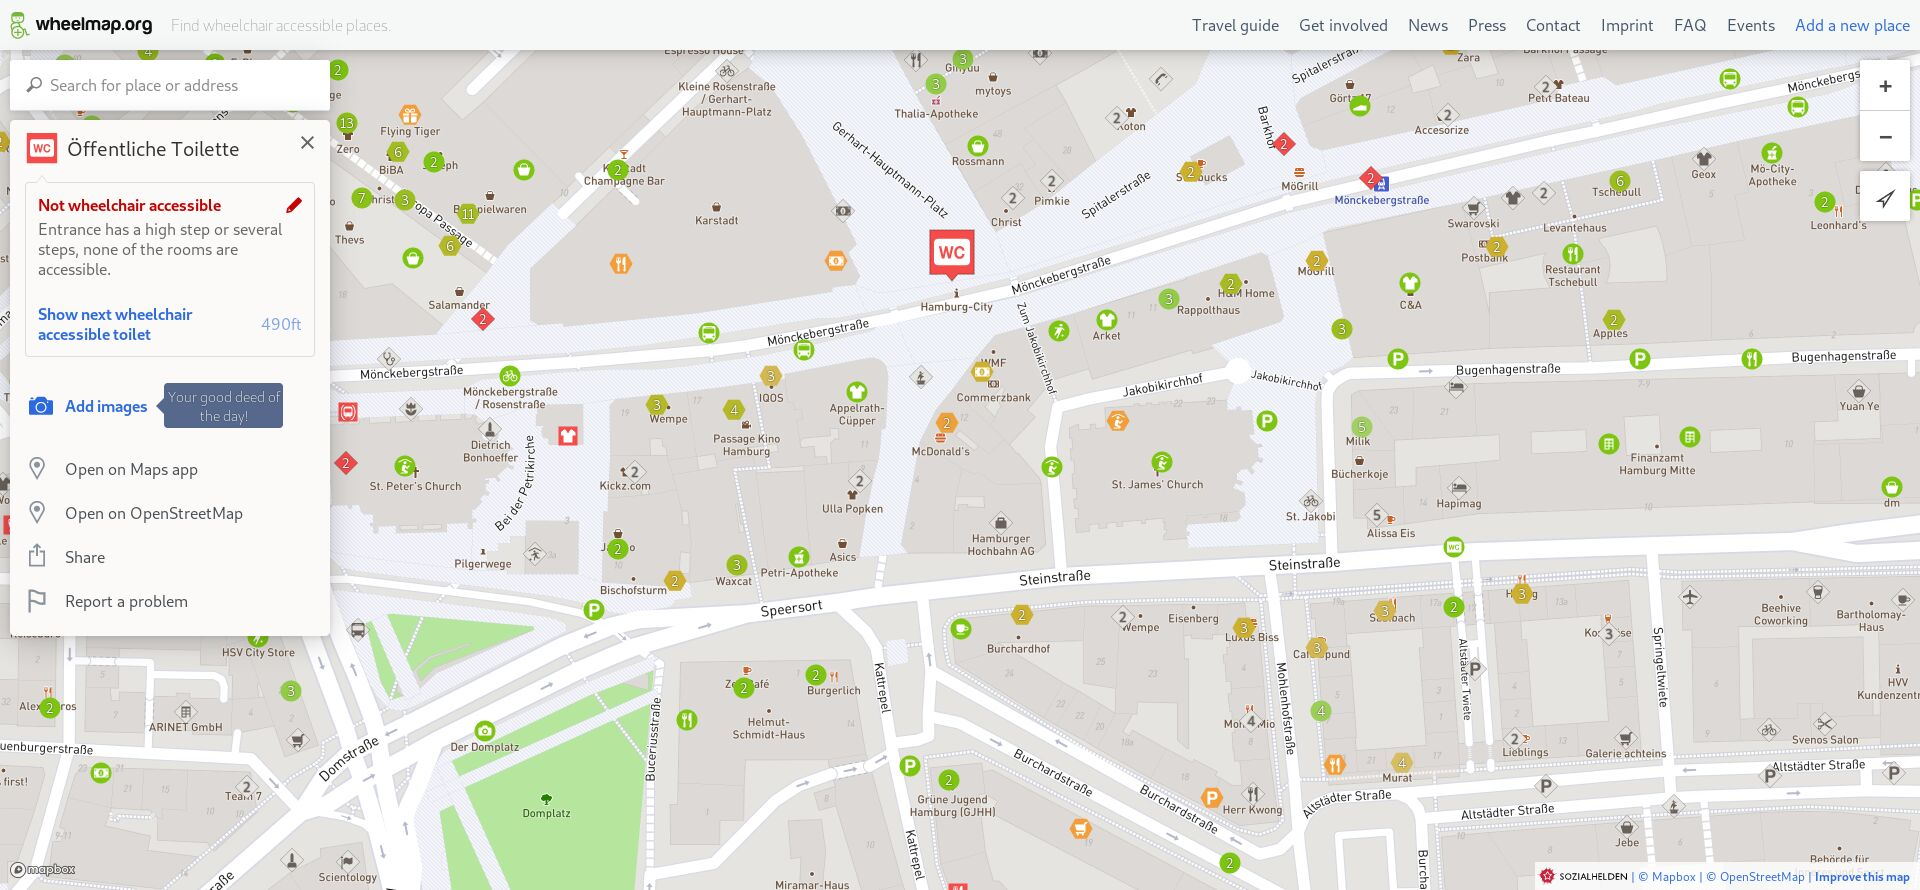
\includegraphics[height=0.7\textheight]{images/wheelmap-website.jpg}\\
					\url{https://wheelmap.org}
				\end{center}
			\end{frame}

		\subsection{Community}
		
			\begin{frame}{What is done?}
				\begin{itemize}
					\item developing software and tools
					\item actual mapping
					\begin{itemize}
						\item going outside collecting data
						\item using external sources (e.g. aerial imagery)
						\item talk to non-mappers (e.g. in schools, local store owners, officials, ...)
					\end{itemize}
					\item creating and maintaining documentation
					\item organizing events (conferences, mapathons, workshops, ...)
				\end{itemize}
			\end{frame}
		
			\begin{frame}{Organization}
				\begin{itemize}
					\item \href{https://wiki.openstreetmap.org/}{wiki}
					\item \href{https://wiki.openstreetmap.org/wiki/Mailing_lists}{mailing lists}
					\item \href{https://community.openstreetmap.org/}{forum}
					\item \href{https://wiki.openstreetmap.org/wiki/Contact_channels}{and more}: discord, telegram, mastodon, reddit, ...)
				\end{itemize}
			\end{frame}

	\section{OSM data}
		
		\begin{frame}
			\tableofcontents[currentsection]
		\end{frame}
		
		\subsection{Tags (attributes)}
		
			\begin{frame}
				\begin{itemize}
					\item simple key-value-pairs (untyped)
					\item free tagging system
					\item standardized by community proposals
					\item central documentation: wiki
				\end{itemize}
				\vspace{0.25cm}
				Multiple strategies:\\
				\vspace{0.25cm}
				\begin{tabular}{|l|l|l|}
					\hline
					\textbf{format} & \textbf{notation} & \textbf{example} \\
					\hline
					normal & \texttt{key=value} & \texttt{highway=service} \\ 
					\hline 
					multiple values & \texttt{key=v1;v2} & \texttt{amenity=library;cafe} \\ 
					\hline 
					namespace & \texttt{namespace:key=value} & \texttt{addr:housenumber=42} \\ 
					\hline 
				\end{tabular}
			\end{frame}
		
		\subsection{Geometries}
		
			\begin{frame}[fragile]{Node (point)}
				\begin{center}
					\begin{columns}
						\begin{column}{1.25cm}
							\centering
							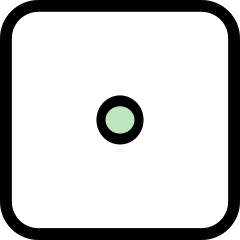
\includegraphics[width=1cm]{images/240px-Mf_node.png}
						\end{column}
						\begin{column}{3.75cm}
							\centering
							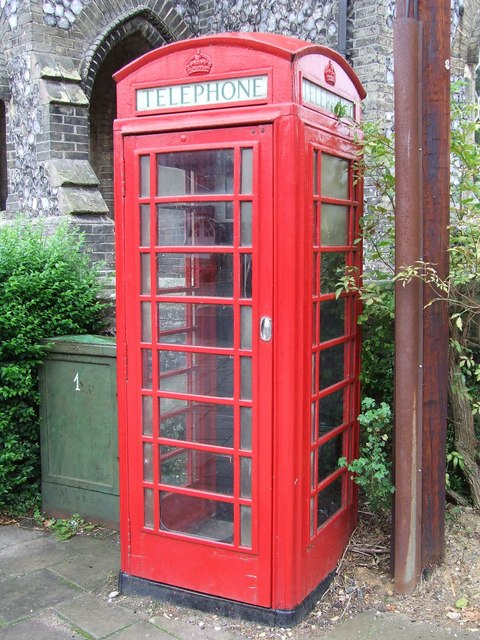
\includegraphics[width=3.5cm]{images/red-telephone-box-uk.jpg}\\
							\textcolor{gray}{
								\tiny
								\href{https://wiki.openstreetmap.org/wiki/File:Red\_telephone\_box\_-\_geograph.org.uk\_-_919348.jpg}{OSM-wiki}
							}
						\end{column}
						\begin{column}{3.5cm}
							\begin{verbatim}
								amenity=telephone
								covered=booth
							\end{verbatim}
							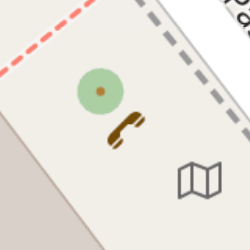
\includegraphics[height=3cm]{images/telephone.png}
						\end{column}
					\end{columns}
				\end{center}
			\end{frame}
		
			\begin{frame}[fragile]{Way (line)}
				\begin{center}
					\begin{columns}
						\begin{column}{1cm}
							\centering
							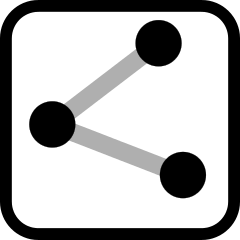
\includegraphics[width=1cm]{images/240px-Mf_way.png}
						\end{column}
						\begin{column}{4.5cm}
							\centering
							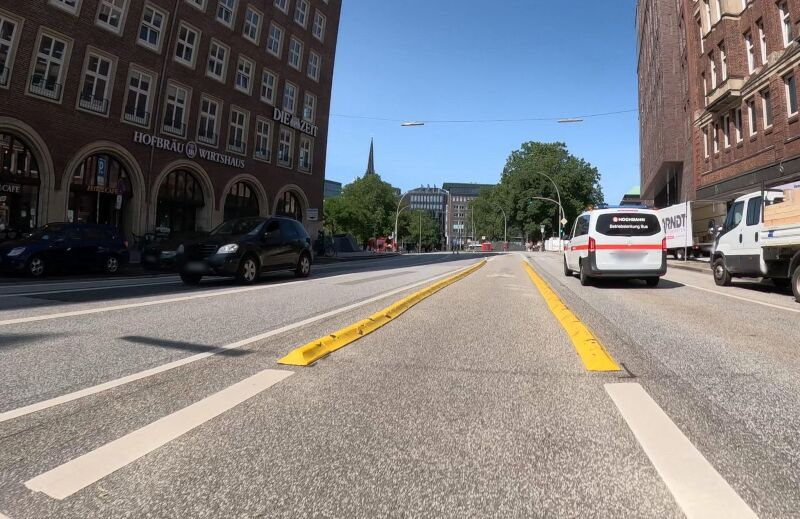
\includegraphics[width=4.5cm]{images/way-example.jpg}
							\textcolor{gray}{
								\tiny
								\href{https://www.mapillary.com/app/?pKey=680503257254203}{Mapillary}
							}
						\end{column}
						\begin{column}{3.5cm}
							\begin{verbatim}
								highway=secondary
								oneway=yes
								name=Speersort
							\end{verbatim}
							\begin{center}
								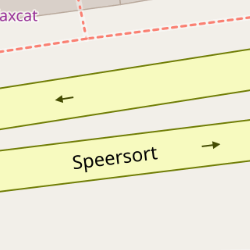
\includegraphics[height=3cm]{images/secondary.png}
							\end{center}
						\end{column}
					\end{columns}
				\end{center}
			\end{frame}
			
			\begin{frame}[fragile]{Area (polygon = closed way)}
				\begin{center}
					\begin{columns}
						\begin{column}{1cm}
							\centering
							
\includegraphics[width=1cm]{images/240px-Mf_area.png}
						\end{column}
						\begin{column}{4.5cm}
							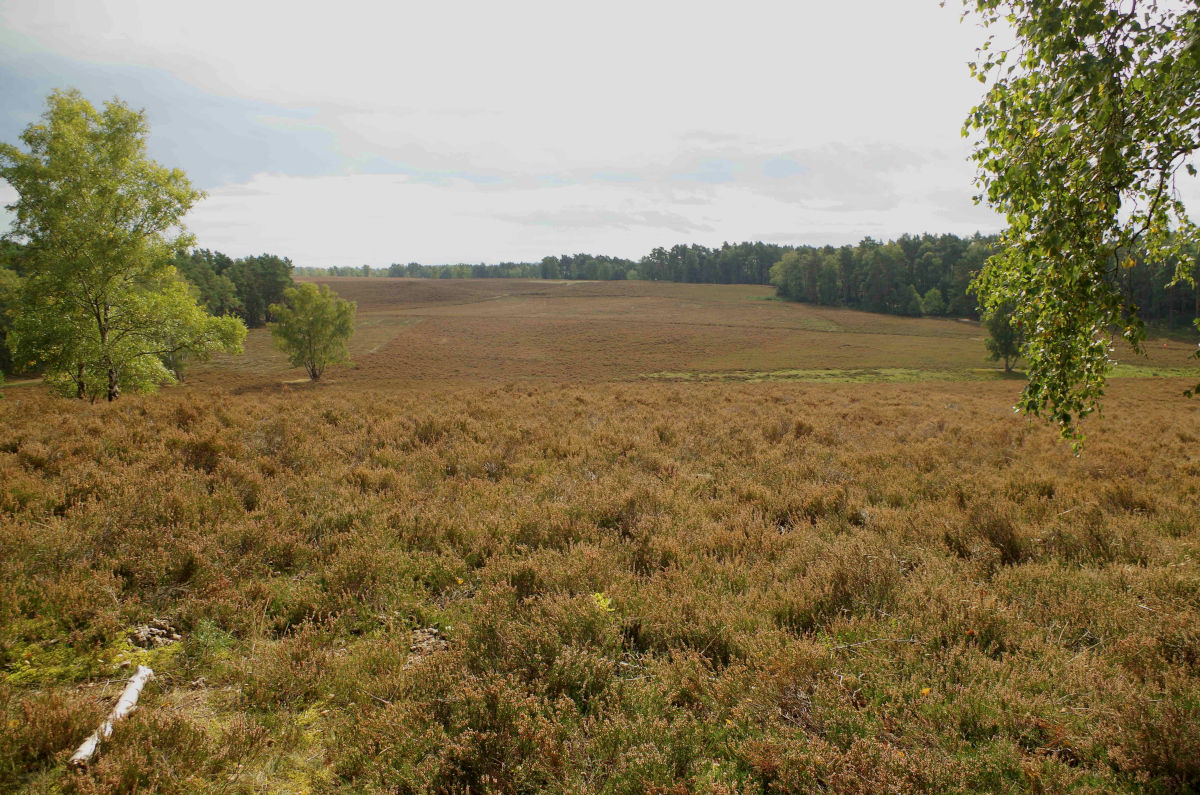
\includegraphics[width=4.5cm]{images/area-example.jpg}
						\end{column}
						\begin{column}{4cm}
							\begin{verbatim}
								natural=heath
								name=Fischbeker Heide
							\end{verbatim}
							\begin{center}
								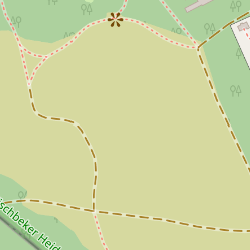
\includegraphics[height=3cm]{images/heath.png}
							\end{center}
						\end{column}
					\end{columns}
				\end{center}
			\end{frame}
	
			\begin{frame}[fragile]{Relation: combine multiple feature into one}
				\begin{center}
					\begin{columns}
						\begin{column}{1.25cm}
							\centering
							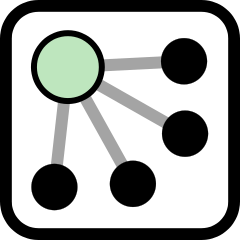
\includegraphics[width=1cm]{images/240px-Mf_relation.png}
						\end{column}
						\begin{column}{4cm}
							\begin{verbatim}
								type=route
								route=bus
								ref=4
							\end{verbatim}
							\vspace{0.25cm}
							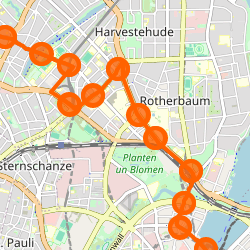
\includegraphics[width=3.75cm]{images/relation-example.png}
						\end{column}
						\begin{column}{4cm}
							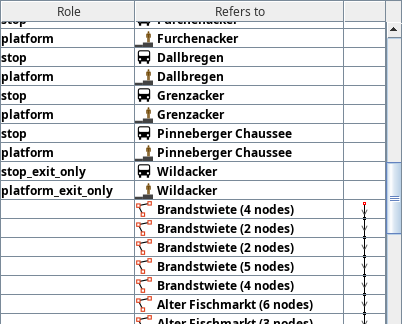
\includegraphics[width=4cm]{images/relation-list.png}
						\end{column}
					\end{columns}
				\end{center}
			\end{frame}
			
			\begin{frame}{Multipolygon (relation; polygon inside polygon)}
				\begin{center}
					\texttt{farmland=center}
					\vspace{0.5cm}
					\begin{columns}
						\begin{column}{4cm}
							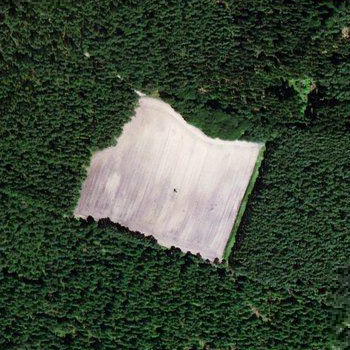
\includegraphics[width=\linewidth]{images/multipolygon-example.png}
						\end{column}
						\begin{column}{4cm}
							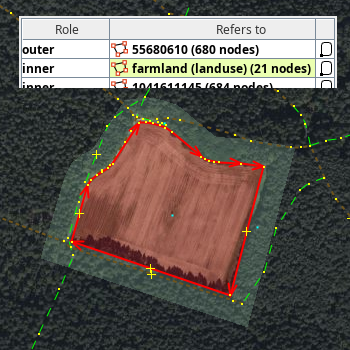
\includegraphics[width=\linewidth]{images/multipolygon-josm.png}
						\end{column}
					\end{columns}
					\vspace{0.25cm}
					\textcolor{gray}{\tiny Imagery: Microsoft\copyright Bing(tm) Maps Platform}
				\end{center}
			\end{frame}
			
			\begin{frame}[fragile]{OSM-XML format}
				OSM uses an XML format (\texttt{.osm} file; often compressed in to a \texttt{.osm.pbf} file):
				\vspace{0.25cm}
				{
					\scriptsize
					\begin{Verbatim}
<?xml version='1.0' encoding='UTF-8'?>
<osm version='0.6' generator='JOSM'>
    <node id='1' action='modify' visible='true' lat='53.558' lon='9.991' />
    <node id='2' action='modify' visible='true' lat='53.548' lon='9.972' />
    <node id='3' action='modify' visible='true' lat='53.545' lon='9.997' />
    <way id='4' action='modify' visible='true'>
        <nd ref='1' />
        <nd ref='2' />
        <nd ref='3' />
    </way>
</osm>
					\end{Verbatim}
				}
			\end{frame}

	\section{Contributing to OSM}
	
		\begin{frame}
			\tableofcontents[currentsection]
		\end{frame}
		
		\subsection{Contributing to OSM}
		
			\begin{frame}{Editing process}
				\begin{enumerate}
					\item register on \href{https://www.openstreetmap.org/user/new}{osm.org}\pause
					\item choose editor
					\begin{itemize}
						\item web: iD
						\item desktop: JOSM
						\item mobile: StreetComplete, OsmAnd, Vespucci
					\end{itemize}\pause
					\item make changes\pause
					\item upload changeset
				\end{enumerate}
			\end{frame}
			
			\begin{frame}{Editors: iD}
				\begin{center}
					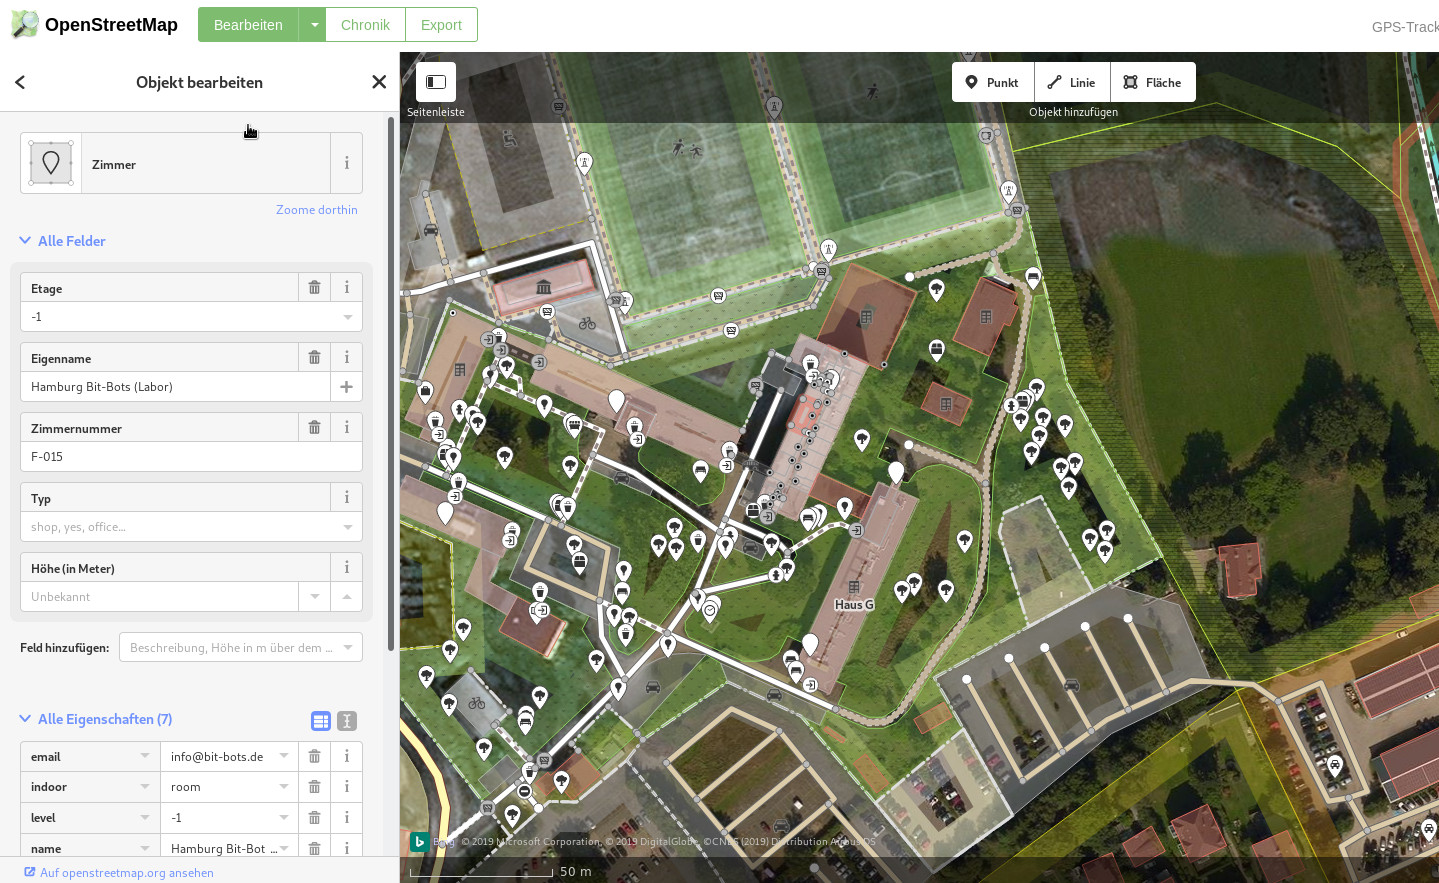
\includegraphics[height=0.75\textheight]{images/id-editor.jpg}
					\href{https://www.openstreetmap.org/edit}{osm.org/edit}
				\end{center}
			\end{frame}
			
			\begin{frame}{Editors: JOSM}
				\begin{center}
					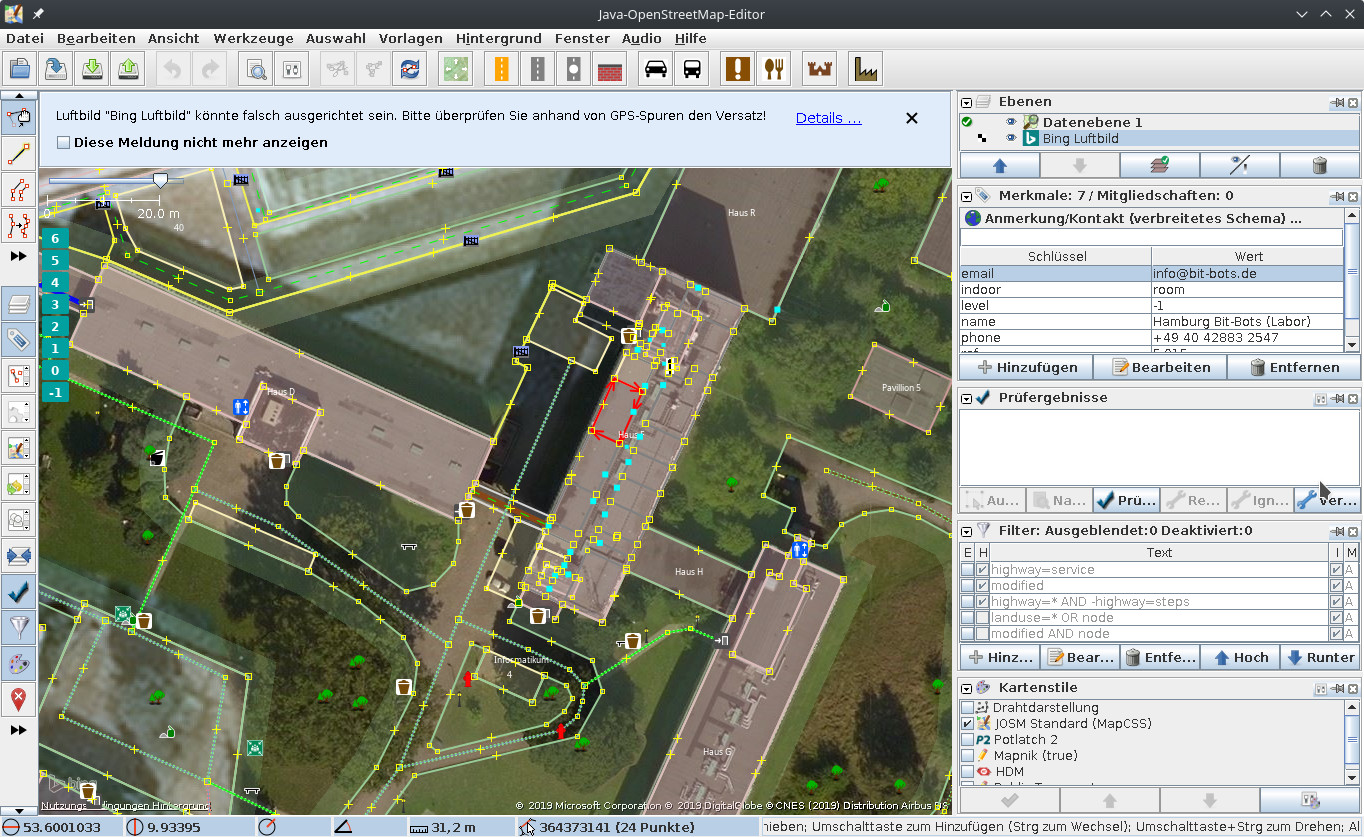
\includegraphics[height=0.75\textheight]{images/josm-editor.jpg}
					\href{https://josm.openstreetmap.de/}{josm.osm.org}
				\end{center}
			\end{frame}
			
			\begin{frame}{Making changes}
				Process for iD and JOSM:
				\begin{enumerate}
					\item collect data (e.g. during hiking)
					\begin{itemize}
						\item make notes, photos, etc.
						\item record GPS tracks
					\end{itemize}\pause
					\item open editor and get raw data\pause
					\item get familiar with tags for your data \textrightarrow\ wiki\pause
					\item add/change/remove existing data\pause
					\item review your changes
				\end{enumerate}
			\end{frame}
			
			\begin{frame}{Collect data}
				\begin{itemize}
					\item make notes while being outside \textleftarrow\ best option!
					\item tracing from imagery (\enquote{armchair mapping})
					\item photos news articles, development plans, etc.
				\end{itemize}
			\end{frame}
			
			\begin{frame}{Using external sources}
				For example:
				\begin{itemize}
					\item imagery (e.g. ESRI World Imagery)
					\item official data (e.g. ALKIS\footnote{Amtliches Liegenschaftskatasterinformationssystem})
					\item photos, websites, etc.
				\end{itemize}
				\pause
				\vspace{0.25cm}
				{
					\setbeamercolor{block title}{bg=orange!65, fg=black}
					\setbeamercolor{block body}{bg=orange!25}
					\begin{block}{Important!}
						Licenses \textbf{must} always be \href{https://wiki.openstreetmap.org/wiki/Import/ODbL_Compatibility}{compatible with the ODbL}! Contact owner if needed!
					\end{block}
				}
			\end{frame}
			
			\begin{frame}{Upload changeset}
				Process for iD and JOSM:
				\begin{enumerate}
					\item review your changes\pause
					\item click the upload/save button\pause
					\item fill in form fields:
					\begin{itemize}
						\item changeset comment: short description of changes
						\item source: source/origin of data (see \href{https://wiki.openstreetmap.org/wiki/Key:source}{wiki} for conventions)
					\end{itemize}\pause
					\item click the upload button
				\end{enumerate}
			\end{frame}
			
			\begin{frame}{Other ways to contribute}
				\begin{itemize}
					\item report errors/missing/outdated data
					\begin{enumerate}
						\item go to osm.org
						\item right click on map \textrightarrow\ \enquote{Add a note here}
						\item enter useful information and save
						\item important: you need an account to write comments
					\end{enumerate}\pause
					\item deal with companies/agencies to obtain permission to use their data\pause
					\item organize events\pause
					\item spread the word
				\end{itemize}
			\end{frame}
	
	\section{Using the data}
	
		\begin{frame}
			\tableofcontents[currentsection]
		\end{frame}
		
		\begin{frame}{The terms of usage}
			Feel free to:
			\begin{itemize}
				\item download the data
				\item use the data (also commercially)
				\item share the data or derivative works (e.g. a printed map)
			\end{itemize}
			Under the following conditions:
			\begin{itemize}
				\item add proper attribution!
				\item keep the data/work under ODbL
				\item do not restrict shared data
			\end{itemize}
		\end{frame}
		
		\begin{frame}{Access the data}
			\begin{itemize}
				\item small areas
				\begin{itemize}
					\item osm.org \textrightarrow\ \enquote{Export} \textrightarrow\ select area \textrightarrow\ \enquote{Export}
					\item API: \href{https://www.openstreetmap.org/api/0.6/map?bbox=9.93116,53.59846,9.93572,53.60052}{\texttt{osm.org/api/0.6/map?bbox=...}}
					\item \href{https://overpass-turbo.eu/}{Overpass API} (filtering and download in various formats)
				\end{itemize}\pause
				\item large areas
				\begin{itemize}
					\item \href{https://download.geofabrik.de/}{Geofabrik GmbH}
					\item everything (\texttt{planet.osm} dump; weekly updated; >70GB OSM-PBF file)
				\end{itemize}
			\end{itemize}
			\pause
			\vspace{0.25cm}
			More in the wiki \textrightarrow\ \href{https://wiki.openstreetmap.org/wiki/Downloading\_data}{Downloading data}.
		\end{frame}
		
		\begin{frame}{Process the data}
			Libraries:
			\begin{itemize}
				\item GDAL, GeoTools: swiss army knifes of geodata processing
				\item libosmium: special OSM-centric library (python \& node bindings)
				\item Leaflet/OpenLayers/MapLibre: display maps/geodata
			\end{itemize}
			\pause
			CLI tools:
			\begin{itemize}
				\item ogr2ogr: part of GDAL to convert formats
				\item osmium: multi-purpose OSM processing CLI tool
				\item osmosis: also powerful but slowly running out of use
				\item osm2pgsql: Import OSM data into a PostGIS database
			\end{itemize}
			\pause
			Desktop applications:
			\begin{itemize}
				\item QGIS: number one open source GIS tool
				\item JOSM: OSM editor, useful for general geodata processing
			\end{itemize}
		\end{frame}
\end{document}












